\section{Implementation}\label{sec:pro1}
In \autoref{chap:concept} wurden Umsetzungsmöglichkeiten für die verschiedenen Bewertungskriterien aus \autoref{sec:criteria} ausgearbeitet.
Diese sollen in die Implementierung des ersten Prototyps einfließen und so einen Grundstein für eine positive Benutzererfahrung der App legen. \\

Der erste Prototyp wurde am 16. Dezember 2017 fertiggestellt und in die bestehende Android-App eingebunden. \\

\noindent
Zusätzlich wurde der Aufbau des Projekts in der \emph{Unified Modelling Language}, kurz \emph{UML}, modelliert.
Dies ermöglicht bereits vor der eigentlichen Implementierung wichtige Begriffe und mögliche Beziehungen festzulegen, und einen Überblick über die benötigten Klassen zu bekommen.

\begin{figure}[h]
  \centering
  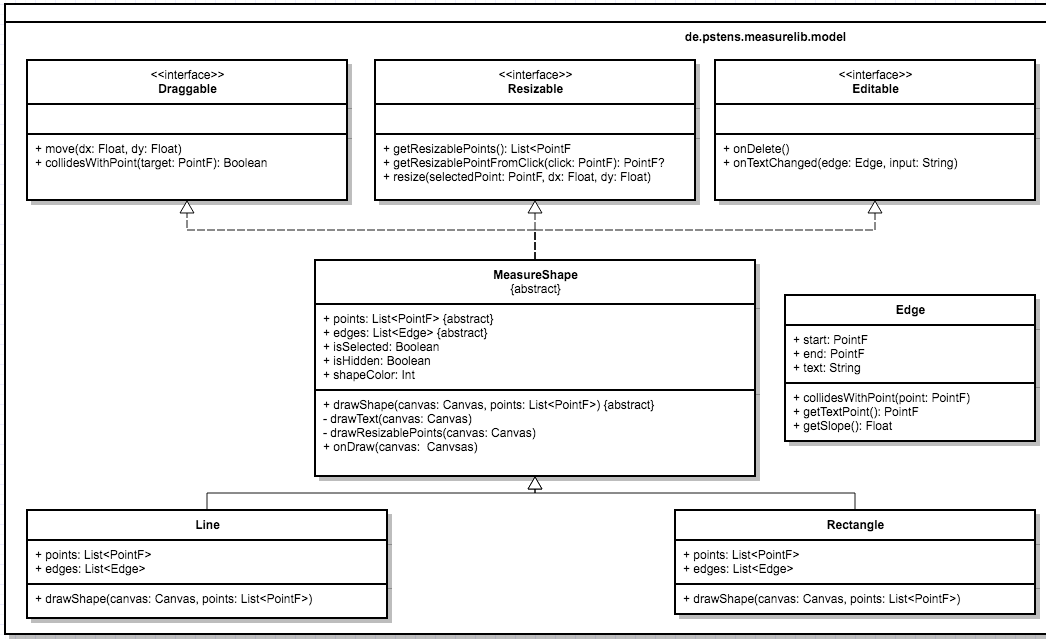
\includegraphics[keepaspectratio, width=\textwidth]{prototype1/shape}
  \caption{Ausschnitt aus der Datenmodell-Komponente des UML-Diagramms}
  \label{fig:shape}
\end{figure}

\noindent
Die Komponente des \emph{Datenmodells} sah dabei wie folgt aus (eine vollständige Version des UML-Diagramms befindet sich in \autoref{chap:uml}):
In \autoref{fig:shape} ist die abstrakte Klasse \emph{MeasureShape} zu erkennen, welche die Oberklasse der beiden Formen \emph{Line} und \emph{Rectangle} darstellt.
\emph{MeasureShape} vererbt die abstrakten Attribute \emph{points} und \emph{edges} an ihre Unterklassen, die diese Attribute überschreiben müssen.
Außerdem muss die öffentliche Methode \emph{drawShape(...)} von beiden Unterklassen implementiert werden.
Dies sorgt dafür, dass jede Unterklasse selber dafür ``verantwortlich'' ist, wie und wohin ihre Form gezeichnet wird.
\emph{MeasureShape} implementiert die drei \emph{Interfaces} \emph{Draggable, Resizable} und \emph{Editable}, welche Schnittstellen zum Verschieben, Vergrößern und Editieren von Formen bereit stellen. \\

\noindent
Eine weitere Klasse im \emph{Datenmodell} ist \emph{UserAction} (siehe \autoref{fig:model}).
Diese ist eine versiegelte (\emph{sealed}) Oberklasse, welche die verschiedenen Benutzeraktionen darstellt.
Versiegelt bedeutet in diesem Kontext, dass nur Klassen, welche im \emph{Scope} der Oberklasse liegen, von dieser erben können.
Folgende sechs Benutzeraktionen können in der Implementierung des ersten Prototyps über die Undo/Redo-Funktion rückgängig gemacht oder wiederhergestellt werden:

\begin{itemize}
  \item Verschieben von Formen (\emph{DraggedShape})
  \item Hinzufügen von Formen (\emph{AddedShape})
  \item Löschen von Formen (\emph{RemovedShape})
  \item Vergrößern bzw. verkleinern von Formen (\emph{ResizedPoint})
  \item Ändern des Textes (\emph{ChangedText})
  \item Ändern der Farbe (\emph{ChangedColor})
\end{itemize}

\noindent
Funktional beschränkt sich die Implementierung des ersten Prototyps zunächst auf das Zeichnen von einfachen Linien und Vierecken, sowie das anschließende Beschriften um Messwerte einzutragen.
Zum schnellen und präzisen Zeichnen der Formen wird eine Zoom-Linse (siehe \autoref{fig:draw1}), wie sie in allen drei Apps aus \autoref{chap:eval} umgesetzt wurde, verwendet.
Der Prototyp verfügt über zwei verschiedene Modi, den Zeichen- und Text-Modus, zwischen denen mit Hilfe des \emph{Floating Action Buttons} im unteren rechten Bildschirmbereich umgeschaltet werden kann (siehe \autoref{fig:all1}).
Zudem kann der Benutzer über einen weiteren \emph{Floating Action Button} im unteren linken Bildschirmbereich jederzeit ein neues Bild aufnehmen, oder ein bereits vorhandenen in die App importieren.

\begin{figure}[h]
  \begin{subfigure}[t]{0.4\textwidth}
    \centering
    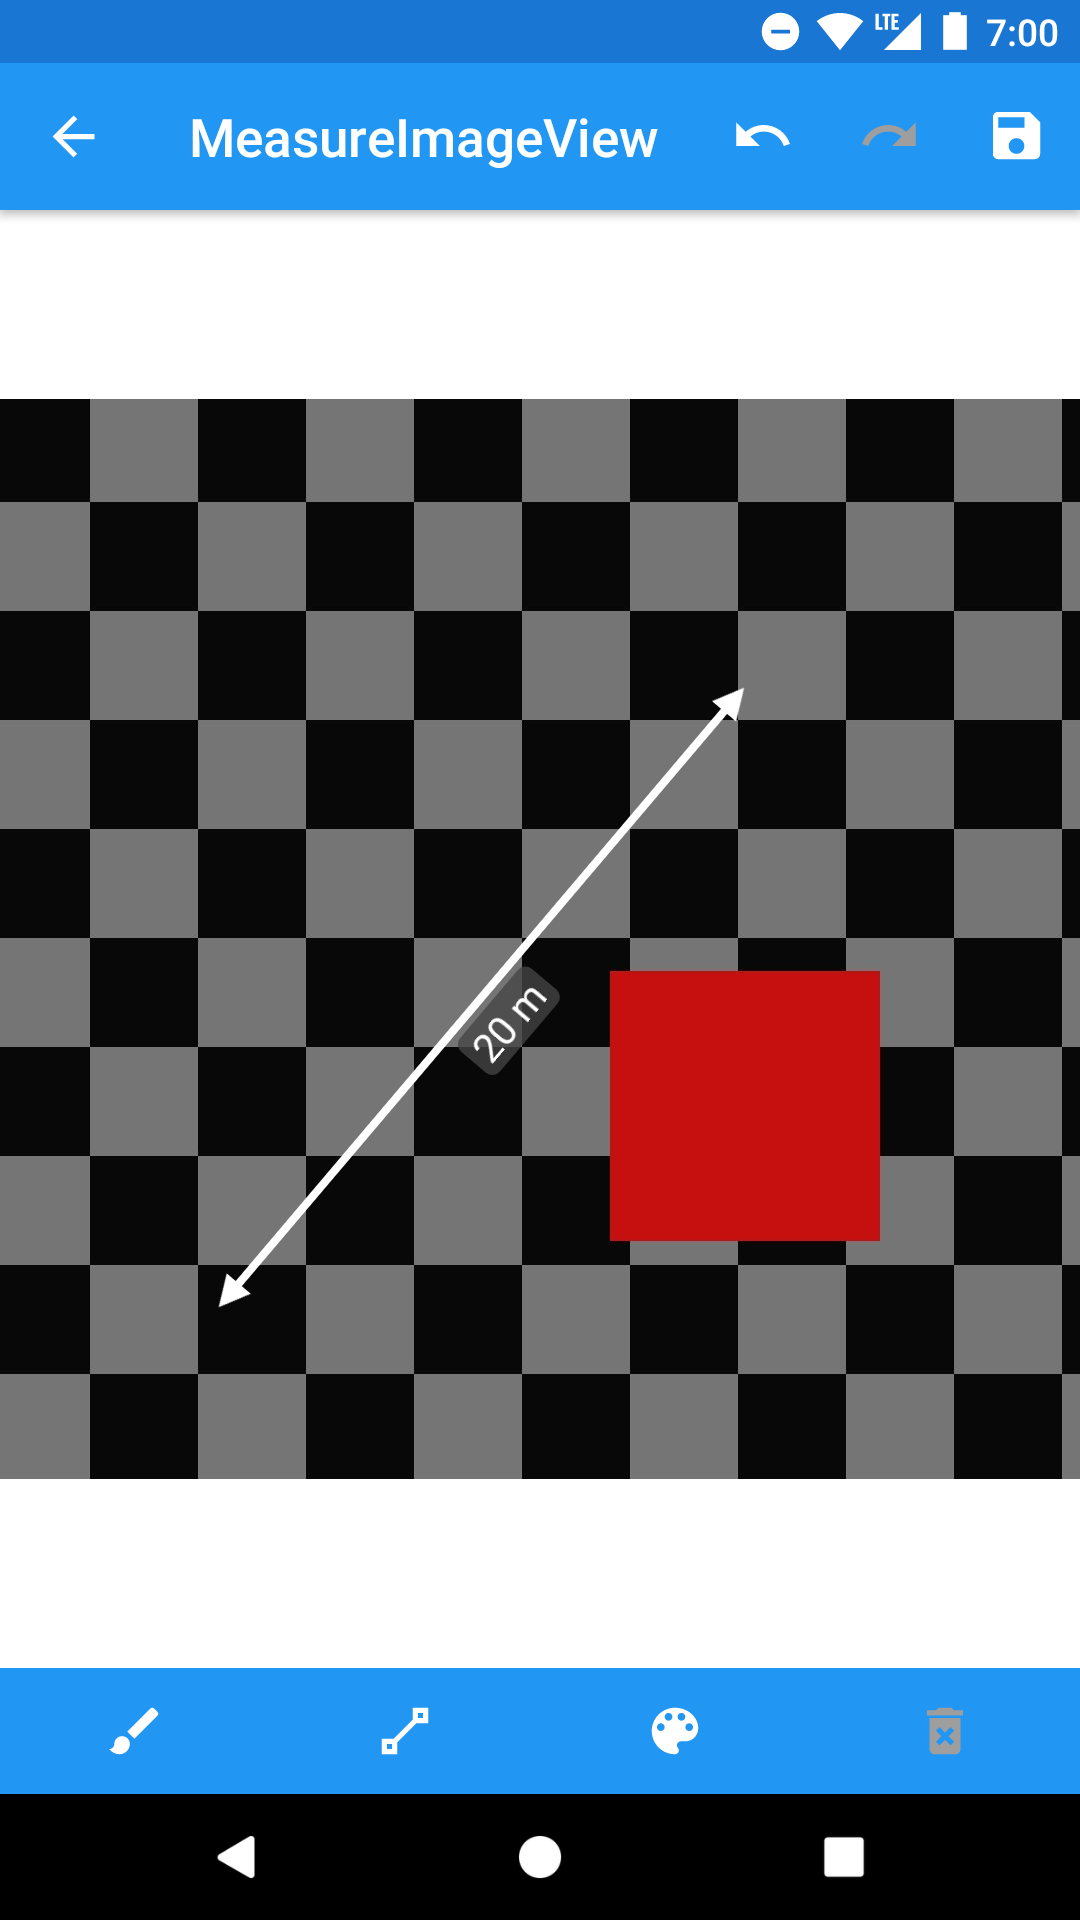
\includegraphics[keepaspectratio, width=\textwidth]{prototype1/all}
    \caption{Erster Prototyp mit bereits eingezeichneter Linie}
    \label{fig:all1}
  \end{subfigure}
  ~
  \begin{subfigure}[t]{0.4\textwidth}
    \centering
    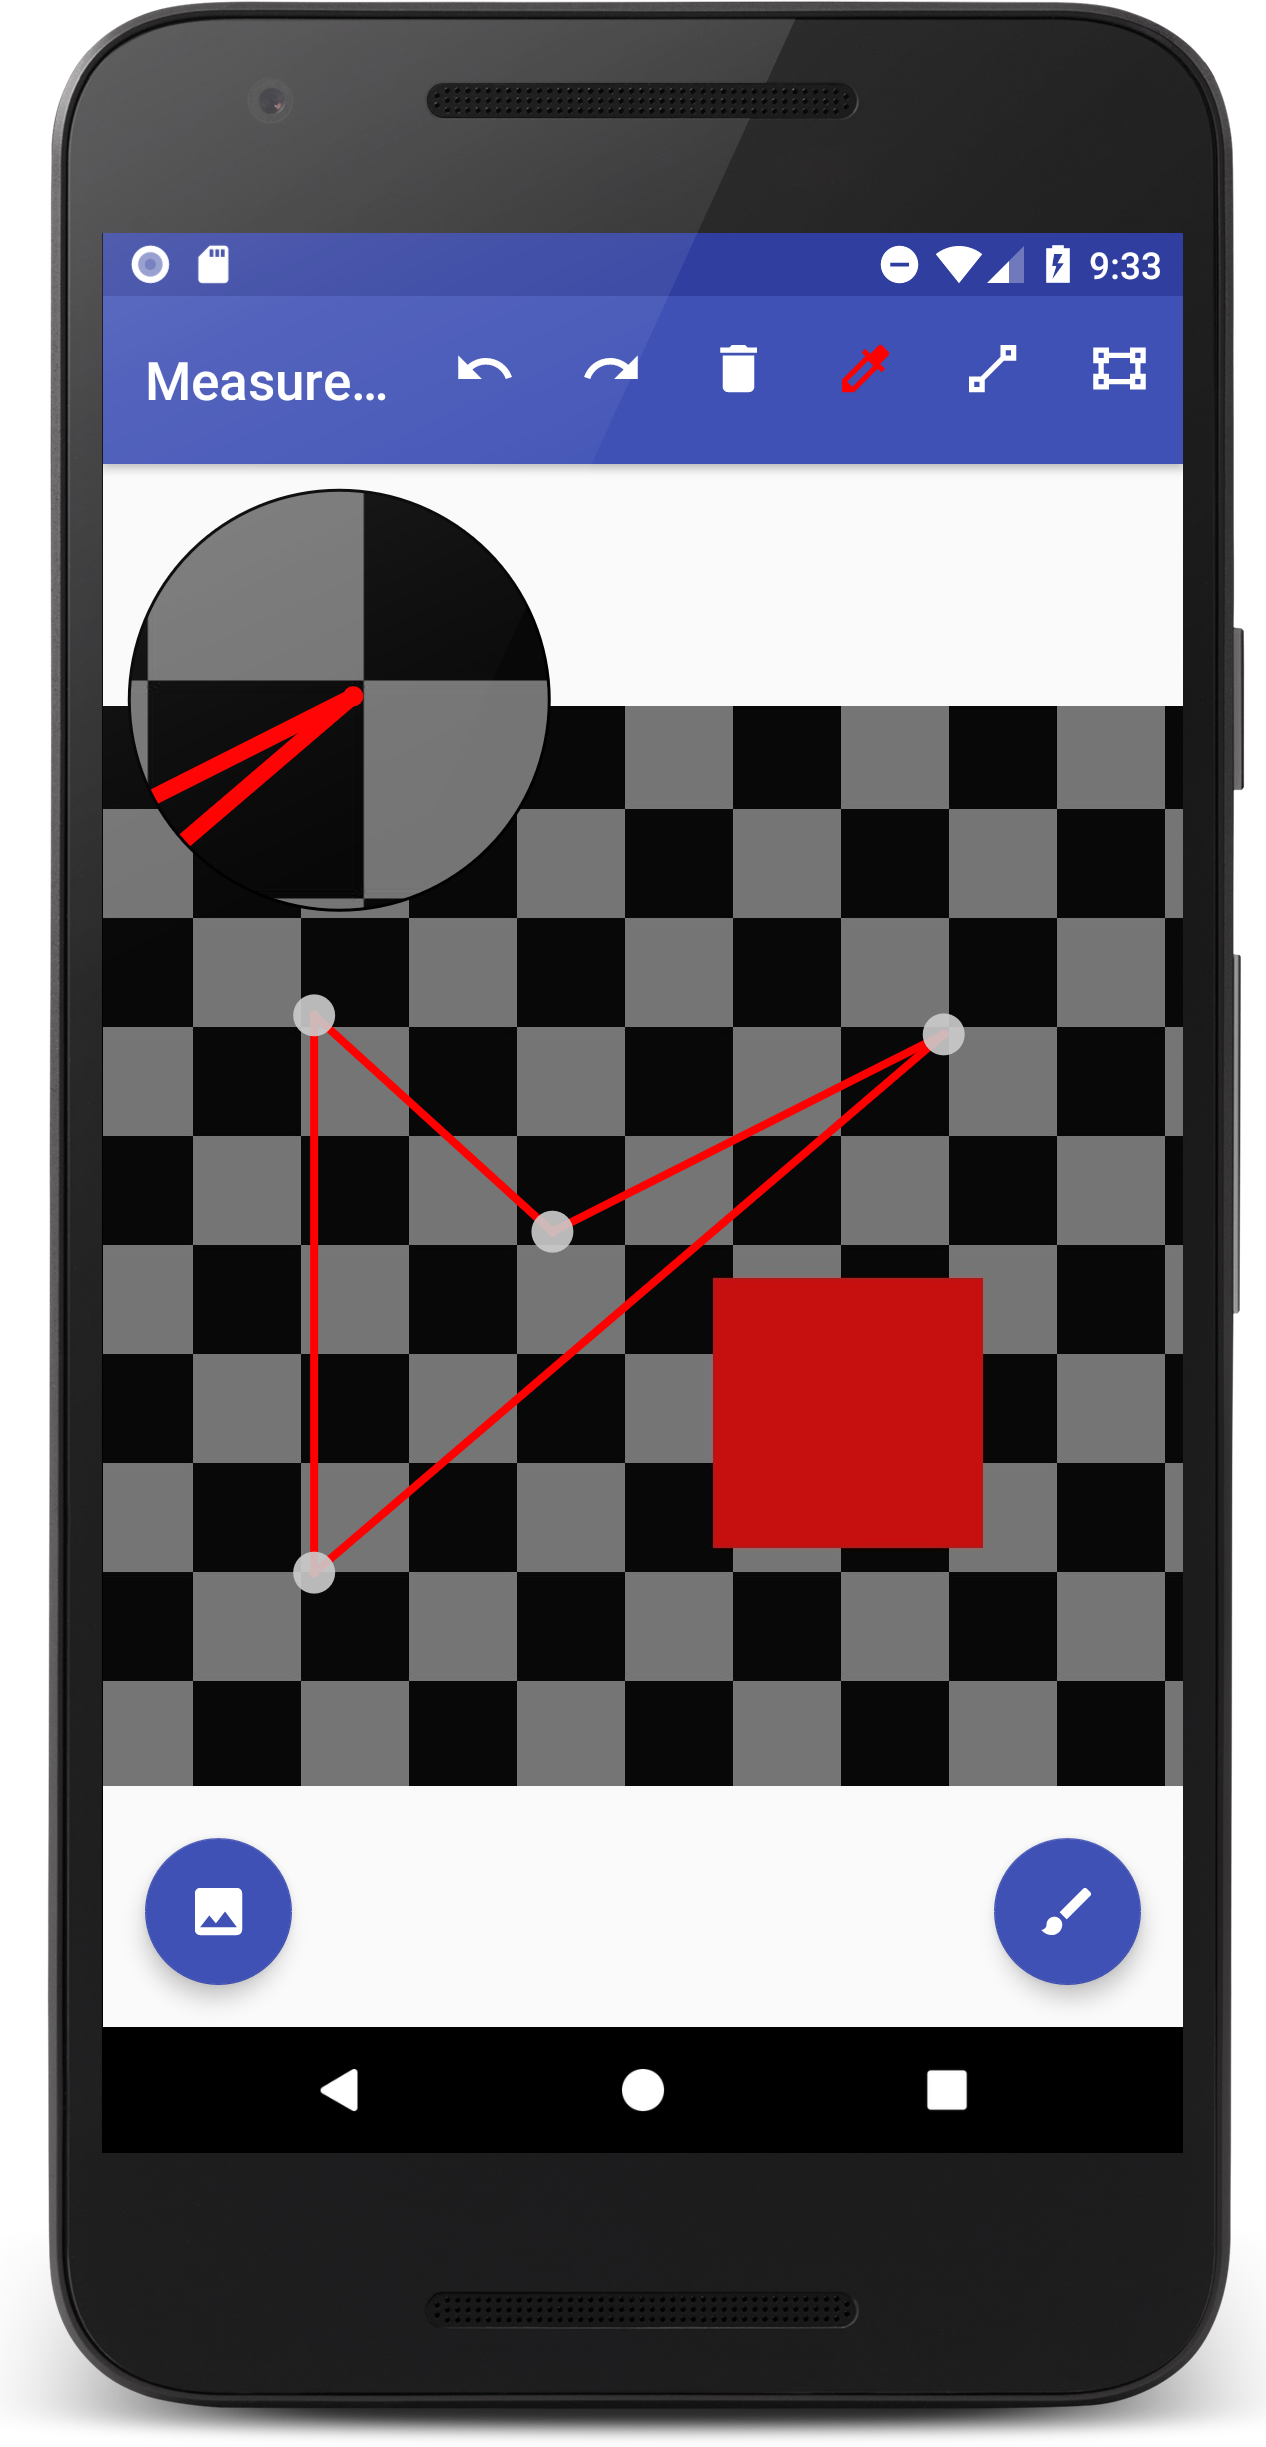
\includegraphics[keepaspectratio, width=\textwidth]{prototype1/rect}
    \caption{Zoom-Linse beim Zeichnen eines Vierecks}
    \label{fig:draw1}
  \end{subfigure}
  \centering
  \caption{Erster Prototyp bei eingezeichneter Linie und beim Zeichnen eines Vierecks}
\end{figure}

Undo- sowie Redo-Funktion befinden auf dedizierten \emph{Buttons} in der Menüleiste der App (siehe \autoref{fig:all1}).
Hier gibt es außerdem jeweils einen Button, um ausgewählte Formen zu löschen, die Zeichenfarbe zu ändern, oder eine andere Form zum Zeichnen auszuwählen. \\

Beim Auswählen des Farb-Icons in der Menüleiste öffnet sich ein modaler Dialog, der es dem Benutzer ermöglicht, die gewünschte Farbe auszuwählen (siehe \autoref{fig:colorpicker}).
Diese Farbe wird als Standardfarbe für alle neuen Formen genutzt.
Falls vor dem Öffnen des Dialogs eine Form markiert wurde, wird diese ebenfalls mit der ausgewählten Farbe eingefärbt. \\

\begin{figure}[h]
  \begin{subfigure}[t]{0.4\textwidth}
    \centering
    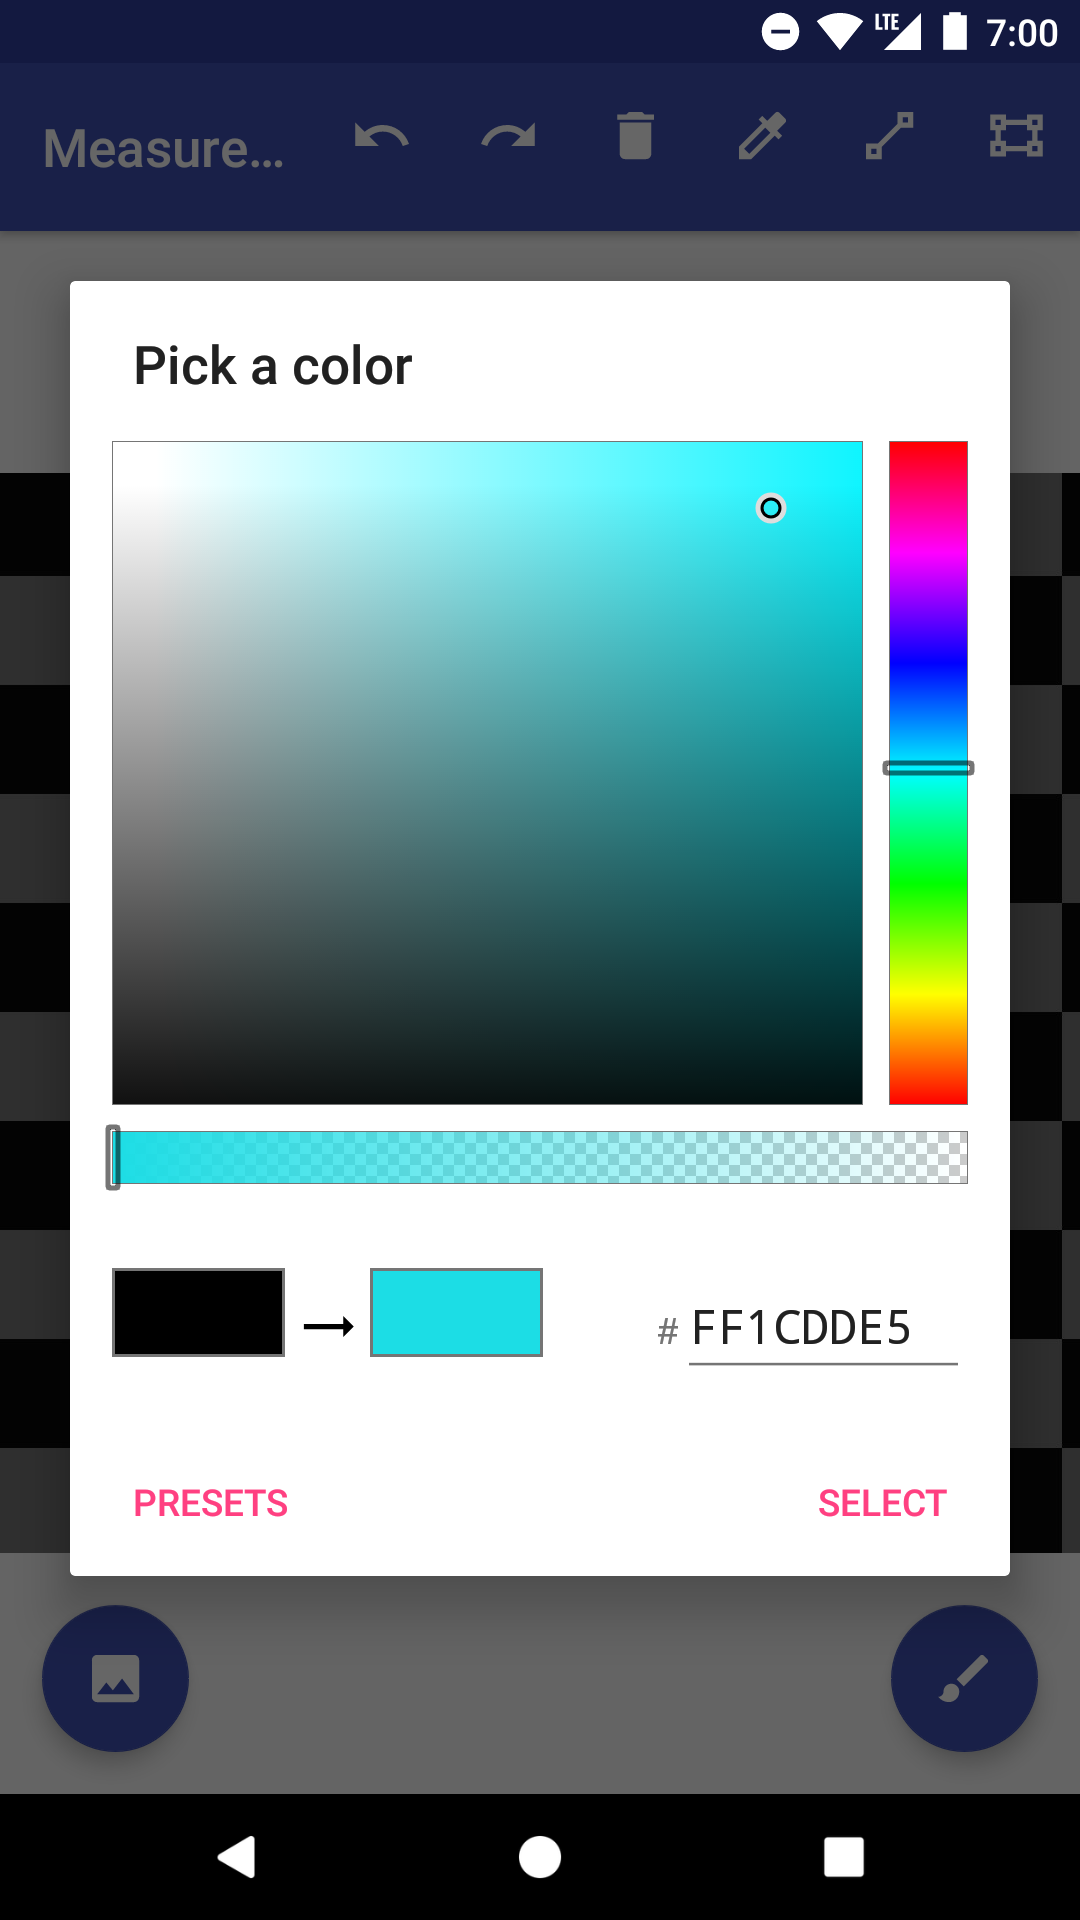
\includegraphics[keepaspectratio, width=\textwidth]{prototype1/color}
    \caption{Geöffneter Farbauswahl-Dialog}
    \label{fig:colorpicker}
  \end{subfigure}
  ~
  \begin{subfigure}[t]{0.4\textwidth}
    \centering
    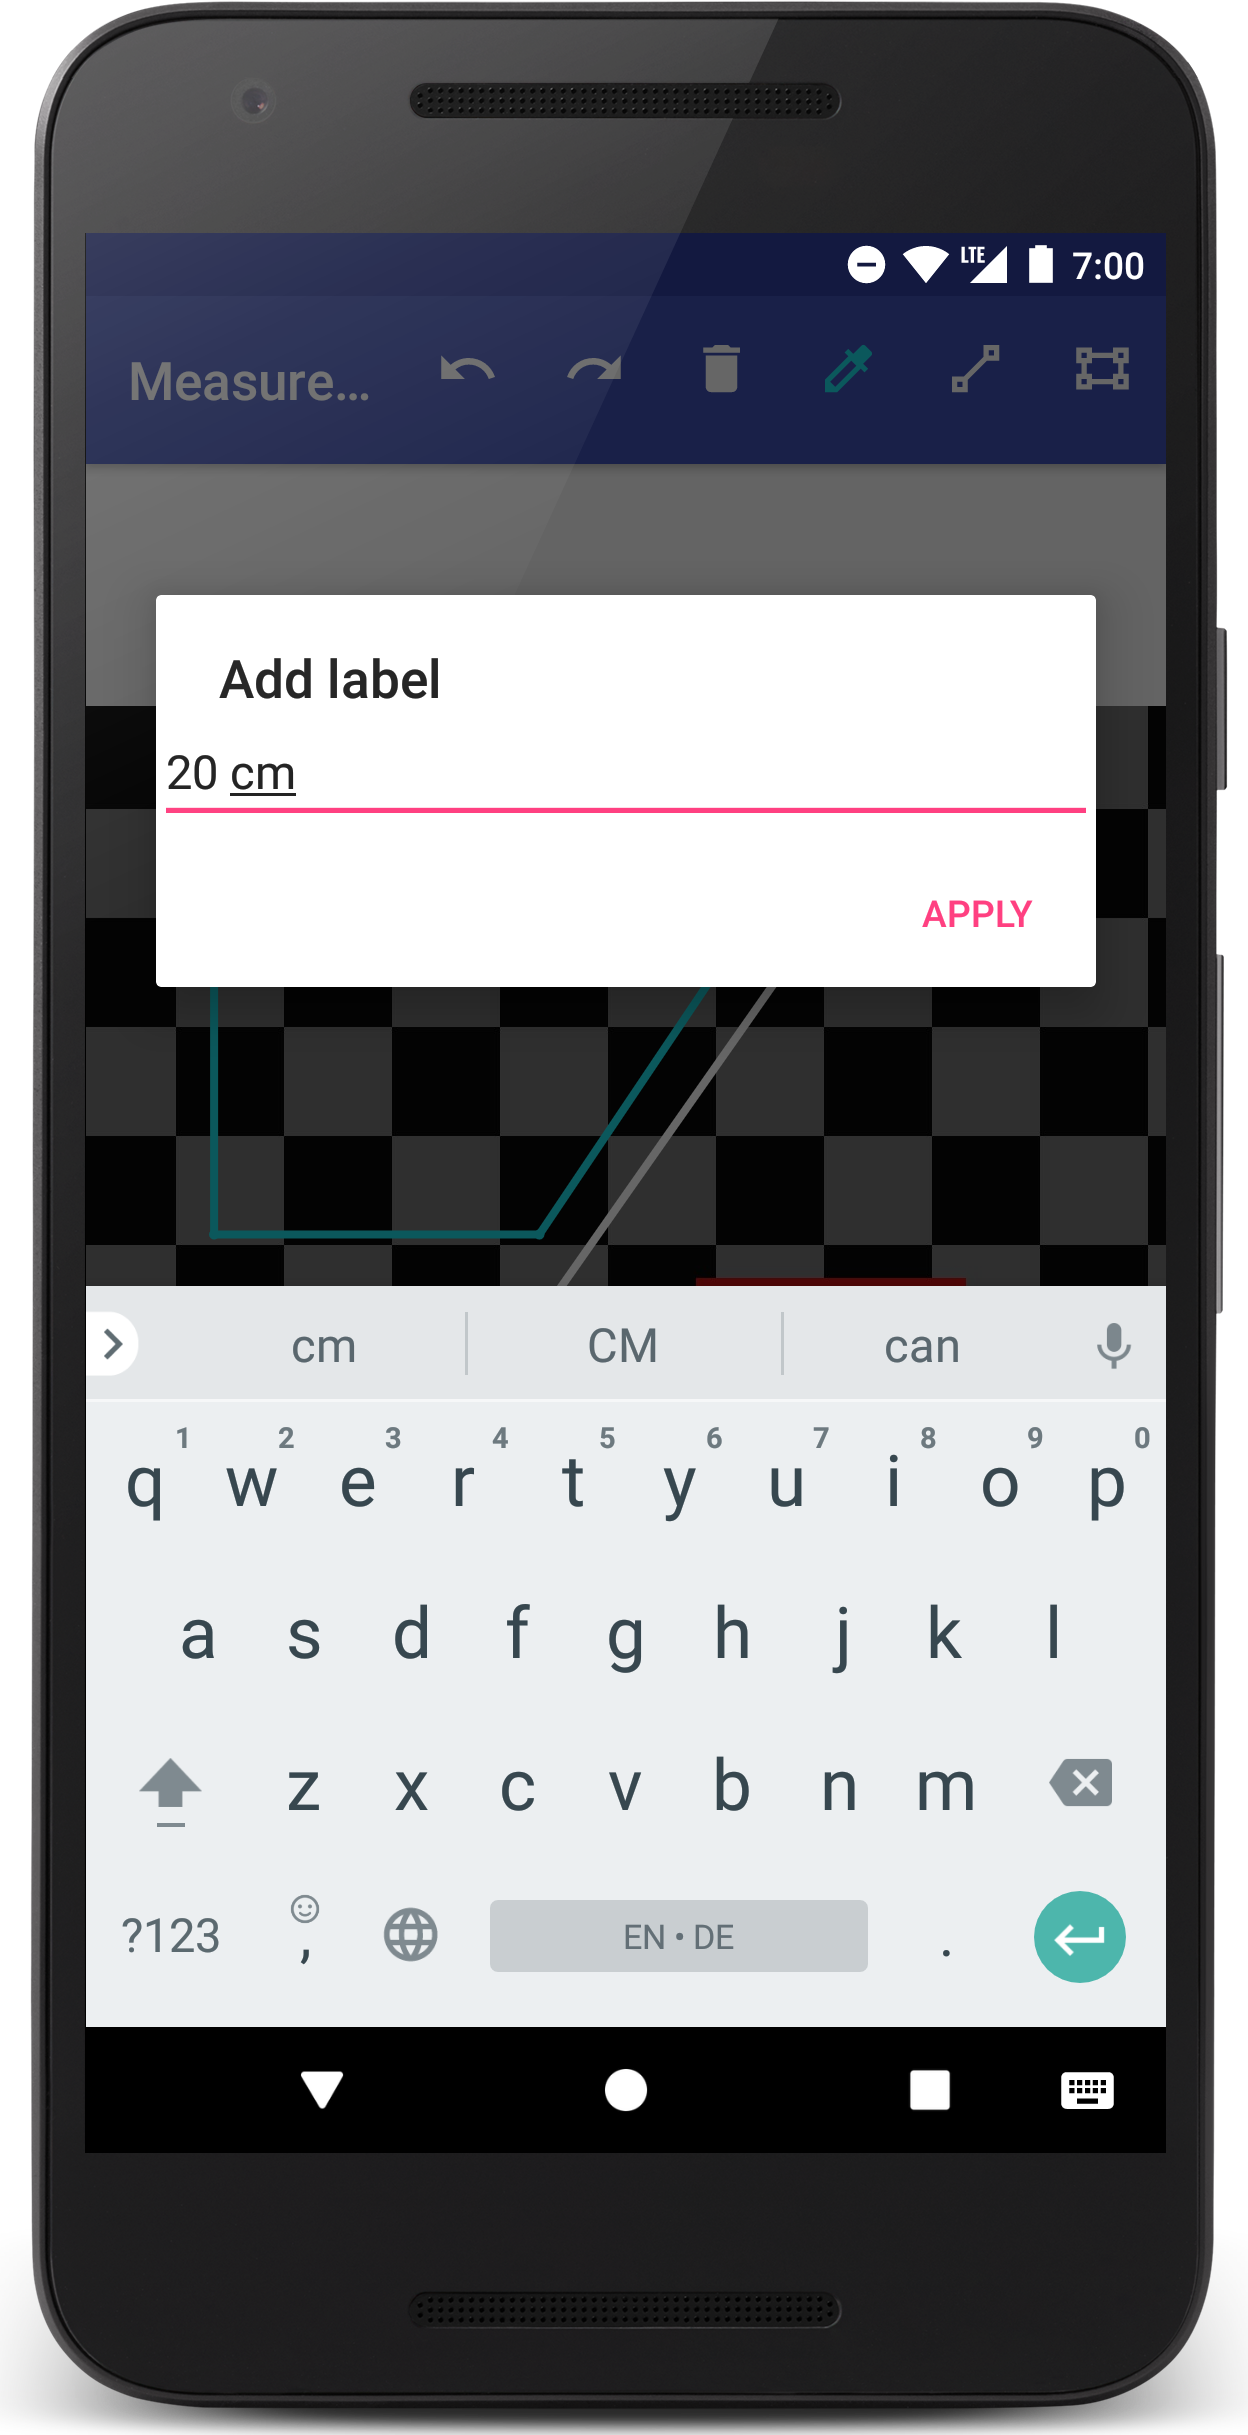
\includegraphics[keepaspectratio, width=\textwidth]{prototype1/labeling}
    \caption{Geöffneter Messwert-Dialog}
    \label{fig:labeling}
  \end{subfigure}
  \centering
  \caption{Erster Prototyp mit geöffnetem Farbauswahl- und Messwert-Dialog}
\end{figure}

Graue Indikatoren an den Eckpunkten der aktuell ausgewählte Form (siehe \autoref{fig:draw1}) sollen dem Nutzer verdeutlichen, dass diese mit Hilfe der Indikatoren in ihrer Größe und Position bearbeitet werden kann.
Um Formen zu beschriften bietet sich dem Benutzer im Text-Modus die Möglichkeit, Kanten mittels eines Eingabe-Dialogs zu annotieren (siehe \autoref{fig:labeling}).
Hierzu öffnet sich durch einen langen Klick auf die Kante einer Form im Text-Modus ein modaler Dialog, welcher die Messwerte des Nutzers entgegennimmt.
Eingetragene Messwerte werden anschließend neben der zuvor ausgewählten Kante im Bild dargestellt. 

\section{Test}\label{sec:test1}
Zum Testen des Prototyps wurde dieser in die App der beiden Geschäftsführer der \emph{Fa.} \vr{} (siehe \autoref{table:testers}) eingebunden.
Testperson 1, André Vermeulen, repräsentiert hierbei den ``Poweruser'' der App, wohingegen Testperson 2, Sebastian Wiesbrock, die App gelegentlich nutzt.
Beiden Testern wurde zur Nutzung des Prototyps weder eine verbale noch schriftliche Hilfestellung zur Verfügung gestellt. \\

\begin{table}[h]
  \centering
  \begin{tabular}{l | c | c}
    \hline
    \textbf{Testperson} & \textbf{1} & \textbf{2} \\
    \hline
    \textbf{Name} & André Vermeulen & Sebastian Wiesbrock \\
    \hline
    \textbf{Rolle} & Geschäftsleitung & Geschäftsleitung \\
    \hline
    \textbf{Alter} & 45 &  ?? \\
    \hline
    \textbf{Nutzungsgrad der App} & hoch & mittel \\
    \hline
  \end{tabular}
  \caption{Demografische Daten der Testpersonen}
  \label{table:testers}
\end{table}

Nachdem die beiden Tester den Prototyp zwei Tage in ihren Arbeitsalltag integriert haben, wurden am 18. Dezember die Testergebnisse gesammelt:

Nach Aussage beider Testpersonen, haben die \emph{Floating Action Buttons} sich bei der Benutzung der App als großes Hindernis herausgestellt.
So sei nicht intuitiv klar, dass die App über zwei verschiedene Modi, nämlich den Zeichen- und Text-Modus, verfügt.
Zudem sei unklar, dass man über einen Klick auf den rechten \emph{Floating Action Button} zwischen den beiden Modi wechseln kann. \\

Ein weiteres Problem ergab sich laut Testperson 1 bei der Benutzung der App auf seinem Tablet.
So seien sämtliche Texte nur schwer lesbar, und die Punkte zum Verändern der Formen so klein, dass sie nur mühsam und mit viel Konzentration mit dem Finger zu treffen seien. \\

Darüber hinaus schilderten beide Testpersonen, dass eingetragene Messwerte auf Bildern, die in dunkleren Lichtverhältnissen aufgenommen wurden, nur schlecht lesbar seien.
Hier setze sich die Textfarbe zu schlecht vom Hintergrund ab. \\

Zusätzlich zu den identifizierten Usability-Problemen kam bei beiden Testern der Wunsch nach neuen Funktionen auf, die sie sich als nützliche Erweiterungen hinsichtlich ihres Arbeitsalltags vorstellen konnten.
So wünschten sich beide Testpersonen einerseits die Möglichkeit, Formen mit bereits vorhandenen Gerüsttypen zu verbinden und in den Meta-Daten des Bildes zu speichern.
Andererseits wurde angemerkt, dass es sinnvoll sei, Bilder vor dem Bearbeiten über eine weitere Oberfläche zunächst in die gewünschte Größe und Form schneiden zu können, da es oftmals auf der Baustelle vorkomme, dass die aufgenommenen Bilder nicht nur das gewünschte Gerüst, sondern auch andere Objekte, die für das Bild nicht relevant sind, beinhalten. \\

Die Ursachen und mögliche Lösungsideen der Probleme, die während dieser Testphase identifiziert wurden, sollen im nächsten Abschnitt in einer weiteren Iteration des \hcdp{} ausgewertet und mit Hilfe eines zweiten Prototyps gelöst werden.
